\documentclass{ctexrep}
\bibliographystyle{plain}
\CTEXsetup[format={\Large\bfseries}]{section}
\usepackage{longtable}
\usepackage{graphicx}
\usepackage{url}
\usepackage{supertabular}
\usepackage{float}
\usepackage{multicol}
\usepackage[a4paper, inner=1.5cm, outer=3cm, top=2cm,bottom=3cm, bindingoffset=1cm]{geometry}
\usepackage{tabularx, makecell, multirow,ulem}
\usepackage[bookmarks=true,colorlinks,breaklinks]{hyperref}
\title{
\rule{16cm}{5pt}\vskip1cm
\textbf{
\Huge 软件需求规格说明
\vspace{0.5cm}
\\ \huge 人群拥塞控制系统
\vspace{0.5cm}
\\ \Large 第三小组
\rule{16cm}{5pt}\vskip1cm
}}
\author{
\begin{tabular}{ll}
 张雨凡 1750219 & 陈恬恬 1751062\\
田云龙 1752248 &李想 1752514\\
罗浩 1752547 & 赵羿昕 1752854 \\
李一珉 1752882 & 张子健 1752894 \\
江宵汉 1752916 & \\
\end{tabular}
}
\date{}

\begin{document}
	\maketitle
	\tableofcontents
\chapter*{版本历史}
\begin{tabular}{|l|p{10cm}|l|}
\hline
\textbf{日期} & \textbf{修改原因} &\textbf{版本号}\\
\hline
\hline
2020.3.30 & 初始版本 & 0.1 \\
\hline
2020.4.1 & 根据展示反馈修改需求工程过程,添加新的参与者与用例,合并一部分旧的用例,添加子系统之间交互关系 & 1.0 \\
\hline
\end{tabular}

\chapter{简介}
本部分将介绍本文档的目的、范围、用词约定、涉及的文献索引以及文档概述。
\section{目的}
本文档的目的在于提供关于人群预警系统的详细描述。本文档将会解释人群预警系统的目的与 特性,它的接口、行为、所受约束与对外界事件的响应。
本文档的主要读者是城市应急处理所对应的职能部门的管理者,本预警系统的开发者团队以及其他潜在的利益相关者。
在经过协商与确认后,本文档将交与各方负责人审核。
\section{范围}
我们的系统是一个「人群拥塞控制系统」,系统的主要目的在于通过多种信息渠道\footnote{包括多媒体、传感器、网络舆情以及前线人员的汇报等等。}收集种种信息,而后与现有的知识库内内容进行对比分析完成预警和处理方案建议。系统将由应急中心的指挥人员、前线人员以及有关的人群拥塞方面的专家团队进行主要的使用和管理,并可以直接向存在潜在危险地区的人民群众发送预警信息。在紧急事件发生后,工作人员可以选择将一定时间范围内的数据进行永久存档,并记录本次事件所采用的处理方式和效果,这些数据将会被用于后续事件的分析。

需要特别注意的是,我们的系统并不仅仅是一个软件系统,我们为前线人员设计了多种专门的设备\footnote{包括款特殊的加密通信设备用于与指挥中心或者公安消防以及急救人员进行联络
、一个便携的显示设备用于查看附近的摄像头或者指挥中心传递的人口热力图等数据
、一个无人机用于给指挥中心传递画面
、一个手持摄像设备用户给指挥中心传递画面
以及其他前线疏散必要的相关设备。} ,并且使用特殊的通信通道来与指挥中心交换信息。
\section{用词约定}
本部分将指出为理解本文档各个部分所需要的各种名词、术语以及缩写方式的定义。这些名词或术语的进一步信息可以从附录或者其他文献中查看。
\begin{longtable}{p{2cm}|p{10cm}}
\hline
用词 & 定义 \\
\hline
\hline
LBS & 基于位置的服务\\
GPS & 全球定位系统 \\
GIS & 地理信息系统 \\
WIFI & 创建于IEEE 802.11标准的无线局域网技术 \\
WIFI辅助定位 & 利用现有的无线网络,配合WIFI标签和相关的移动终端设备再结合相应的定位算法,来确定相关人员和物品位置的一种新技术 \\
必须 & 系统必须要达成的目标,否则将造成失败 \\
希望 & 开发团队希望可以达成的目标,失败将造成用户的失望 \\
尝试 & 开发团队后期可能进行的额外工作,成功将引起用户满意程度较大上升,失败不会有副作用 \\
\hline
\end{longtable}
\section{参考文献}

\section{文档概述}
本文档的剩余部分将会分成两个大的章节以及附录。第二章将会描述针对本系统的功能以及本系统与其他系统的交互的概述,该章也会引入不同类型的利益相关者以及他们与本系统的交互以及本系统在构建过程中所采取的限制与假设。第三章将会对需求进行详细的描述以期较为完整的描述本系统的诸多方面。附录中将会较为详细的叙述我们的需求获取过程,记录我们的利益相关者的用户故事并描述我们在需求工程中的需求诱导以及需求验证的过程中所采取的方法。



\chapter{概述}
本章将会对整个系统进行概述,系统将会在对其对主要功能对描述以及其与其他系统的交互的描述中显现自身,我们也将会描述各种利益相关者对本系统的需求,最后系统的限制和假设也将在本章被描述。
\section{产品观点}
随着我国社会生活的日益丰富,在城市公共场所举办的大型政治、文化、体育、宗教、民俗等方面的活动逐渐增多,同时也带来了一系列的安全隐患,其中最为突出的便是人群发生拥挤而导致的踩踏等群死群伤事故。大型活动中的拥挤踩踏事故是一个多因素、多变量、多层次的复杂系统。在该系统中,除活动场所等环境特征外,参与活动的人群个体的心理与行为也存在着各种不确定性和复杂性。
\begin{figure}[H]
	\centering
	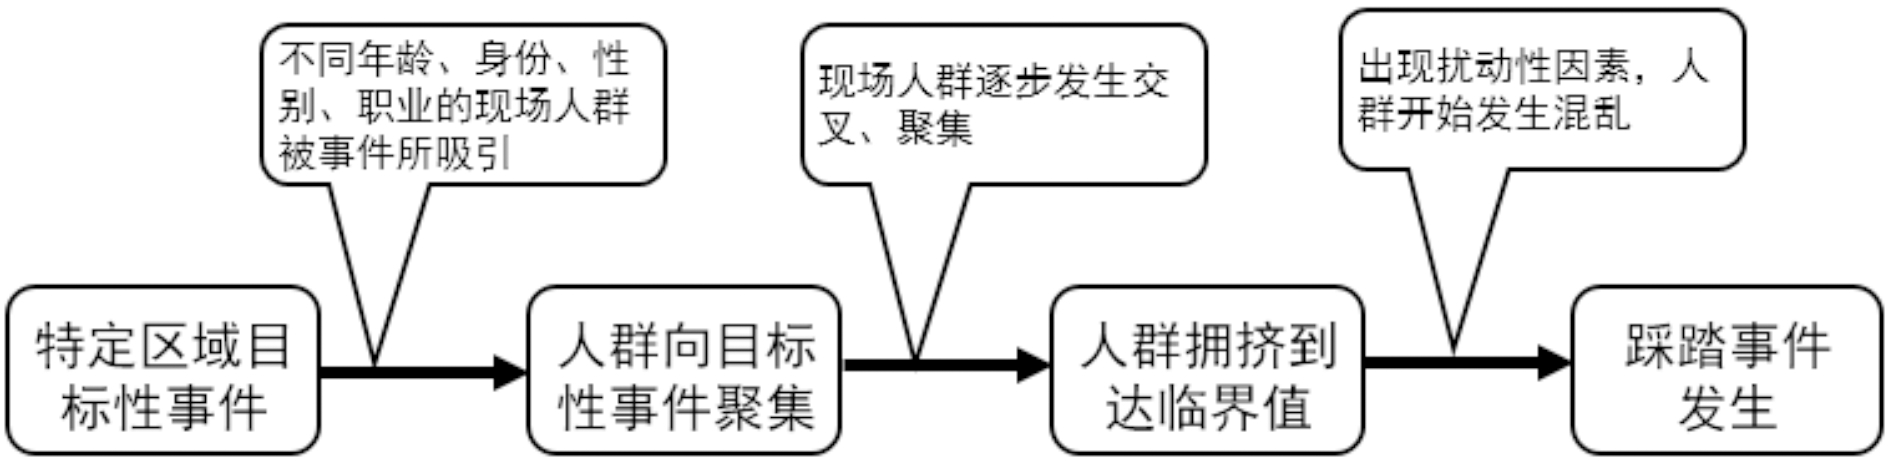
\includegraphics[scale=0.2]{img/stages.png}
	\caption{人群聚集事件的产生过程}
\end{figure}
\section{产品功能}
\section{用户特征}
\section{系统约束}
\section{假设与依赖}


% add other chapters and sections to suit
\end{document}
